%! TeX program = lualatex
% http://www.personal.ceu.hu/tex/latex.htm

\documentclass[11pt,a4paper]{article}
%\usepackage{lua-visual-debug}

\usepackage{pgfplots}
\usepackage{marginnote}
\usepackage{amsmath}
\usepackage{xspace}

\usepackage{array}
\usepackage{tabularx}
\usepackage{booktabs}
\usepackage[ampersand]{easylist}

\usepackage{wrapfig}
% Prevent dropping images by a line in wrapfig
\usepackage{etoolbox}

\makeatletter
\patchcmd\WF@putfigmaybe{\lower\intextsep}{}{}{\fail}%
%\AddToHook{env/wrapfigure/begin}{\setlength{\intextsep}{0pt}}
\makeatother

\usepackage{floatflt}

\usepackage{datatool}
\usepackage{hyperref}
\usepackage{float}
\usepackage{ifthen}
\usepackage[inline]{enumitem}
\hypersetup{pdfborderstyle={/S/U/W 1}}
\usepackage[toc]{glossaries}
\usepackage[marginparwidth=2.3cm]{geometry}
\usepackage{calc}

\usetikzlibrary{angles,arrows.meta,decorations.markings,calc}

\setlength\parindent{0pt}
\date{\today}

\title{L2 Physics Notes}
\author{Ben Tomlin}

\makeglossaries

\tikzset{
	vec/.style={very thick,-{Stealth}},
	cpt/.style={postaction=decorate,decoration={markings, mark=at position 0.5 with {\arrow{>>}}}}
}

\newcommand{\mc}[1]{\pgfmathparse{#1}\pgfmathresult}
\begin{document}
\maketitle

\begin{abstract}
This document is a overview of and reference for the physics concepts at NCEA L2 and the mathematical equations that describe them. 
\end{abstract}


\tableofcontents

\part{Foundations}
\section{Definitions}
The clearer you are about what a word (term) means the better your understanding will be. Some words in physics do not
have the meaning you are used to. Therefore it is important to look up definitions of words and you will have a greater
understanding. See the glossary.

\section{Vectors \& Scalars}

\def\mylsp{1.8}
\newlength\lsp\setlength{\lsp}{\mylsp ex} % label spacing for vectors given as x,y shift
\pgfmathparse{sqrt(\mylsp^2/2)}
\newlength\lspx\setlength{\lspx}{\pgfmathresult ex} % label spacing for vectors given as x,y shift
\newcommand{\vcc}[2]{
	\vcenter{\hbox{\tikz{
				\draw[vec] (0,0) -- (#1:#2);
				\draw[cpt] (0,0) -- (#1:#2 |- 0,0);
				\draw[cpt] (#1:#2|-0,0) -- (#1:#2);
			\draw ($(0,0)!.5!(#1:#2)+({mod(#1+360+90,360)<180?-\lspx:\lspx},{mod(#1+360,360)<180?\lspx:-\lspx})$) node{$V$};
			\draw ($(0,0)!.5!(#1:#2|-0,0) + (0,{mod(#1+360,360)>180?\lsp:-\lsp})$) node{$V_x$};
			\draw ($(#1:#2)!.5!(#1:#2|-0,0)+ ({mod(#1+360+90,360)<180?\lsp:-\lsp},0)$) node {$V_y$};
			}
	}}
}

\newcommand{\vcl}[3]{
	\vcenter{\hbox{\begin{tikzpicture}[vec/.style = {very thick, -{Stealth}}]
		\draw[vec] (0,0) -- (#1:#2) ;
		\draw ($(0,0)!0.5!(#1:#2) + ({90+#1}:2ex)$) node{#3};
	\end{tikzpicture}}}
}



\newcommand{\vadd}[4]{\vaddl{#1}{#2}{A}{#3}{#4}{B}}
\newcommand{\vaddl}[6]{ \vaddll{#1}{#2}{#3}{#4}{#5}{#6}{#3+#6} }
\newcommand{\vaddll}[7]{
	\vcenter{\hbox{\tikz[vec/.style ={very thick, -{Stealth}},line join=miter]{
		\draw[vec,blue] (0,0) -- (#1:#2);
		\draw[vec,blue] (#1:#2) -- ++(#4:#5);
		\draw[red,cpt] (0,0) -- ($(#1:#2)+(#4:#5)$) node(R){};
		
		% When theta of result (R) 0<\theta<180. below{A,B}, above{R}. Else reverse of this
		\draw ($(0,0)!0.5!(#1:#2) + ({#1+(#2*sin(#1)+#5*sin(#4)>0?90:-90)}:-\lsp)$) node{#3};
		\draw ($(#1:#2)!0.5!(R) + ({#4+(#2*sin(#1)+#5*sin(#4)>0?90:-90)}:-\lsp)$) node{#6};
		\draw ($(0,0)!0.5!(R) + ({#4+(#2*sin(#1)+#5*sin(#4)>0?-90:90)}:-\lsp)$) node{#7};
	}}}
}

\newcommand{\vdef}[2]{
	\begin{tikzpicture}[> = Straight Barb, vec/.style ={very thick, -{Stealth}}]
		\draw[vec] (0,0) -- (#1:#2);
		\draw[thin] (0,0) -- (#2,0);

		\draw[shift={(#1+90:0.5ex)},rotate=90] (0,0) -- (#1:3ex) node[pos=0.9](l1){};
		\draw[shift={($(#1+90:0.5ex)+(#1:#2)$)},rotate=90] (0,0) -- (#1:3ex) node[pos=0.9](l2){};

		\draw[ultra thin,<->] (l1.center) -- (l2.center) node[above,midway]{$l$};

		\draw[<->] (#2/4,0) arc(0:#1:#2/4) node[shape=circle,pos=0.5](a){};
		\draw (a.30) node[]{$\theta$};
	\end{tikzpicture}
}


\newglossaryentry{scalar}{name=scalar,description={a number or quantity, only}}
\newglossaryentry{vector}{name=vector,description={a number/size \emph{and} a direction}}

\paragraph{\Glspl{scalar}}
are numbers also called a 'size'. Size is given as a number and unit. It is sometimes also
called a 'length'.

\begin{wrapfigure}{r}{0pt}
	\vdef{45}{2}
\end{wrapfigure}

\paragraph{\Glspl{vector}} 
are a number/size \emph{and} direction. The direction is often given as an angle from the
horizontal. In the diagram to the right, the vector drawn has a length/size/number of $l$ and direction of $\theta\deg$ from the horizontal. 


\subsection{Combining Vectors}
Vector \textbf{do not} add like scalars. Because they have a direction. Vectors can be added and subracted from one
another. To add two vectors, the head of one must be stuck to the tail of the other.
\begin{align*}
	( \vcl{0}{2}{A} + \vcl{45}{2}{B} ) = ( \vcl{45}{2}{B} + \vcl{0}{2}{A} ) = \vadd{0}{2}{45}{2}
\end{align*}
When adding scalars, the answer is a \textit{scalar} and called the \textit{result}. When adding vectors the answer is a
\textit{vector} and called the \textit{resultant}.

\subsection{Negative Vectors}
A negative vector has its direction reversed. $ -1\times(\vcl{36}{2}{A}) = \vcl{36}{-2}{-A} $\\

\begin{wrapfigure}{r}{0pt}$-1\times(\vcl{0}{-1}{C})=\vcl{0}{1}{-C} $\end{wrapfigure}
A negative vector \textbf{does not} point in the negative direction of an axis (ex 'x axis'). It points in the \emph{opposite} direction of it's positive self.

\subsection{Subracting Vectors}
To subtract B from A, we add -B to A
\begin{align*}
	\large  \vcl{0}{2}{A} - \vcl{45}{2}{B} = \vcl{0}{2}{A} + \vcl{45}{-2}{-B}  =
\vadd{0}{2}{45}{-2}
\end{align*}

Note that $A-B \neq B-A$. For any two vectors to be the same they must have the same direction and length.
\begin{align*}
	\vadd{0}{2}{45}{-2} \neq \vadd{45}{2}{0}{-2}
\end{align*} 
These are different resultants because they have different directions (they are opposite). 


\subsection{Vector Components}
\newglossaryentry{component}{name=component,description={a part of an object or thing}}

A vector $V$ can be split into a horizontal ($V_x$) and vertical ($V_y$) \gls{component}. $\vcc{60}{2}$

$V_x$ and $V_y$ are also vectors. They add to the original vector. 
\begin{align*}
	( \vcl{0}{1}{$V_x$} + \vcl{90}{1.7321}{$V_y$} ) = \vaddll{0}{1}{$V_x$}{90}{1.7321}{$V_y$}{$V_x+V_y$} = \vcc{60}{2}
\end{align*}
%$\v\vaddll{0}{1}{$V_x$}{90}{1.7321}{$V_y$}{$V_x+V_y=V$}$

We say $V_x$ and $V_y$ are components of $V$.

\part{Motion}

\section{Motion}
Describe motion of objects in two dimensions.

\begin{description}
	\item[Vectors] Vectors, a direction and size. Addition and subtracting. Components.
	\item[Forces] Forces. How they produce an acceleration. Newtons laws.
	\item[Displacement, Velocity, Acceleration] Used to describe an objects motion.
	\item[Relative Velocity] Describing an objects velocity as seen by a moving observer. 
\end{description}

\subsection{Kinematics}
\marginnote{\textbf{constant} means unchanging. Is a stationary objects acceleration constant?}
The kinematic equations describe motion of an object that has a \textbf{constant} or \textbf{average} acceleration. \\


When an object is accelerating over a time period, its velocity will change between the start of that time period and
the end (unless acceleration is zero). Also, the object will travel some distance during this time. Kinematic
equations relate these quantities. \\

\reversemarginpar 
\marginnote{
	\textbf{averaged} means that the quantity sits at an average value. At a given instant however, it may be greater or
	lesser than the average\\

	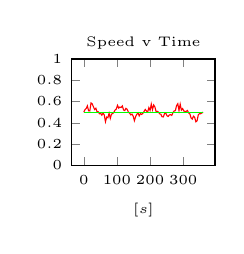
\begin{tikzpicture}
		\begin{axis}[
			xlabel={[$s$]},
			title={\tiny Speed v Time},
			tiny,
			ymin=0,ymax=1,
			width=3.4cm,
			legend style={nodes={scale=0.7}}
		]
		\addplot[
			domain=0:360,
			samples=100,
			color=red,
		] {0.5+0.1*rnd*sin(x*4)};
		\addplot[
			domain=0:360,
			samples=2,
			color=green,
		] {1/2};
	\end{axis}
\end{tikzpicture}
}
\normalmarginpar
Importantly, they are used only when acceleration is \textbf{constant} or \textbf{averaged}.

Kinematic equations are used with \emph{only one direction at a time}. What do we mean by direction? $V_i, V_f, a$ are all
\textbf{vectors} and thus have a \emph{direction}. This means that these must all have a matching direction - ie; all horizontal
or all vertical.

\paragraph{Equations}
\noindent
{\Large
	\begin{eqnarray}
		V_f=V_i+at \\
		d=\frac{V_i+V_f}{2}t \\
		V_f^2=V_i^2+2ad \\
		d=V_it+\frac{at^2}{2}
	\end{eqnarray}
}

\noindent
\begin{tabular*}{\columnwidth}{|c l @{\extracolsep{\fill}} c|}
	\toprule
\textbf{Symbol} & \textbf{Meaning} & \textbf{[Unit]} \\ \midrule
	\(V_i\) & Initial velocity. The velocity at the beginning of a time period. &\(ms^{-1}\) \\
	\(V_f\) & Final velocity, or the velocity at the end of a time period. & \(ms^{-1}\) \\ 
	a & Constant (or average) acceleration for the time period. & \(ms^{-2}\) \\
	t & Time period over which velocity canged. & \(s\) \\
	d & Distance that the object travel(s,led) (in the time period) & m \\ \bottomrule
\end{tabular*}


\part{Forces}

\part{Energy}

\part{Momentum}

\printglossaries
\label{gls}
\end{document}
